
%% bare_jrnl.tex
%% V1.4b
%% 2015/08/26
%% by Michael Shell
%% see http://www.michaelshell.org/
%% for current contact information.
%%
%% This is a skeleton file demonstrating the use of IEEEtran.cls
%% (requires IEEEtran.cls version 1.8b or later) with an IEEE
%% journal paper.
%%
%% Support sites:
%% http://www.michaelshell.org/tex/ieeetran/
%% http://www.ctan.org/pkg/ieeetran
%% and
%% http://www.ieee.org/

%%*************************************************************************
%% Legal Notice:
%% This code is offered as-is without any warranty either expressed or
%% implied; without even the implied warranty of MERCHANTABILITY or
%% FITNESS FOR A PARTICULAR PURPOSE! 
%% User assumes all risk.
%% In no event shall the IEEE or any contributor to this code be liable for
%% any damages or losses, including, but not limited to, incidental,
%% consequential, or any other damages, resulting from the use or misuse
%% of any information contained here.
%%
%% All comments are the opinions of their respective authors and are not
%% necessarily endorsed by the IEEE.
%%
%% This work is distributed under the LaTeX Project Public License (LPPL)
%% ( http://www.latex-project.org/ ) version 1.3, and may be freely used,
%% distributed and modified. A copy of the LPPL, version 1.3, is included
%% in the base LaTeX documentation of all distributions of LaTeX released
%% 2003/12/01 or later.
%% Retain all contribution notices and credits.
%% ** Modified files should be clearly indicated as such, including  **
%% ** renaming them and changing author support contact information. **
%%*************************************************************************


% *** Authors should verify (and, if needed, correct) their LaTeX system  ***
% *** with the testflow diagnostic prior to trusting their LaTeX platform ***
% *** with production work. The IEEE's font choices and paper sizes can   ***
% *** trigger bugs that do not appear when using other class files.       ***                          ***
% The testflow support page is at:
% http://www.michaelshell.org/tex/testflow/



\documentclass[journal]{IEEEtran}
%
% If IEEEtran.cls has not been installed into the LaTeX system files,
% manually specify the path to it like:
% \documentclass[journal]{../sty/IEEEtran}





% Some very useful LaTeX packages include:
% (uncomment the ones you want to load)


% *** MISC UTILITY PACKAGES ***
%
%\usepackage{ifpdf}
% Heiko Oberdiek's ifpdf.sty is very useful if you need conditional
% compilation based on whether the output is pdf or dvi.
% usage:
% \ifpdf
%   % pdf code
% \else
%   % dvi code
% \fi
% The latest version of ifpdf.sty can be obtained from:
% http://www.ctan.org/pkg/ifpdf
% Also, note that IEEEtran.cls V1.7 and later provides a builtin
% \ifCLASSINFOpdf conditional that works the same way.
% When switching from latex to pdflatex and vice-versa, the compiler may
% have to be run twice to clear warning/error messages.






% *** CITATION PACKAGES ***
%
%\usepackage{cite}
% cite.sty was written by Donald Arseneau
% V1.6 and later of IEEEtran pre-defines the format of the cite.sty package
% \cite{} output to follow that of the IEEE. Loading the cite package will
% result in citation numbers being automatically sorted and properly
% "compressed/ranged". e.g., [1], [9], [2], [7], [5], [6] without using
% cite.sty will become [1], [2], [5]--[7], [9] using cite.sty. cite.sty's
% \cite will automatically add leading space, if needed. Use cite.sty's
% noadjust option (cite.sty V3.8 and later) if you want to turn this off
% such as if a citation ever needs to be enclosed in parenthesis.
% cite.sty is already installed on most LaTeX systems. Be sure and use
% version 5.0 (2009-03-20) and later if using hyperref.sty.
% The latest version can be obtained at:
% http://www.ctan.org/pkg/cite
% The documentation is contained in the cite.sty file itself.






% *** GRAPHICS RELATED PACKAGES ***
%
\ifCLASSINFOpdf
  % \usepackage[pdftex]{graphicx}
  % declare the path(s) where your graphic files are
  % \graphicspath{{../pdf/}{../jpeg/}}
  % and their extensions so you won't have to specify these with
  % every instance of \includegraphics
  % \DeclareGraphicsExtensions{.pdf,.jpeg,.png}
\else
  % or other class option (dvipsone, dvipdf, if not using dvips). graphicx
  % will default to the driver specified in the system graphics.cfg if no
  % driver is specified.
  % \usepackage[dvips]{graphicx}
  % declare the path(s) where your graphic files are
  % \graphicspath{{../eps/}}
  % and their extensions so you won't have to specify these with
  % every instance of \includegraphics
  % \DeclareGraphicsExtensions{.eps}
\fi
% graphicx was written by David Carlisle and Sebastian Rahtz. It is
% required if you want graphics, photos, etc. graphicx.sty is already
% installed on most LaTeX systems. The latest version and documentation
% can be obtained at: 
% http://www.ctan.org/pkg/graphicx
% Another good source of documentation is "Using Imported Graphics in
% LaTeX2e" by Keith Reckdahl which can be found at:
% http://www.ctan.org/pkg/epslatex
%
% latex, and pdflatex in dvi mode, support graphics in encapsulated
% postscript (.eps) format. pdflatex in pdf mode supports graphics
% in .pdf, .jpeg, .png and .mps (metapost) formats. Users should ensure
% that all non-photo figures use a vector format (.eps, .pdf, .mps) and
% not a bitmapped formats (.jpeg, .png). The IEEE frowns on bitmapped formats
% which can result in "jaggedy"/blurry rendering of lines and letters as
% well as large increases in file sizes.
%
% You can find documentation about the pdfTeX application at:
% http://www.tug.org/applications/pdftex





% *** MATH PACKAGES ***
%
%\usepackage{amsmath}
% A popular package from the American Mathematical Society that provides
% many useful and powerful commands for dealing with mathematics.
%
% Note that the amsmath package sets \interdisplaylinepenalty to 10000
% thus preventing page breaks from occurring within multiline equations. Use:
%\interdisplaylinepenalty=2500
% after loading amsmath to restore such page breaks as IEEEtran.cls normally
% does. amsmath.sty is already installed on most LaTeX systems. The latest
% version and documentation can be obtained at:
% http://www.ctan.org/pkg/amsmath





% *** SPECIALIZED LIST PACKAGES ***
%
%\usepackage{algorithmic}
% algorithmic.sty was written by Peter Williams and Rogerio Brito.
% This package provides an algorithmic environment fo describing algorithms.
% You can use the algorithmic environment in-text or within a figure
% environment to provide for a floating algorithm. Do NOT use the algorithm
% floating environment provided by algorithm.sty (by the same authors) or
% algorithm2e.sty (by Christophe Fiorio) as the IEEE does not use dedicated
% algorithm float types and packages that provide these will not provide
% correct IEEE style captions. The latest version and documentation of
% algorithmic.sty can be obtained at:
% http://www.ctan.org/pkg/algorithms
% Also of interest may be the (relatively newer and more customizable)
% algorithmicx.sty package by Szasz Janos:
% http://www.ctan.org/pkg/algorithmicx




% *** ALIGNMENT PACKAGES ***
%
%\usepackage{array}
% Frank Mittelbach's and David Carlisle's array.sty patches and improves
% the standard LaTeX2e array and tabular environments to provide better
% appearance and additional user controls. As the default LaTeX2e table
% generation code is lacking to the point of almost being broken with
% respect to the quality of the end results, all users are strongly
% advised to use an enhanced (at the very least that provided by array.sty)
% set of table tools. array.sty is already installed on most systems. The
% latest version and documentation can be obtained at:
% http://www.ctan.org/pkg/array


% IEEEtran contains the IEEEeqnarray family of commands that can be used to
% generate multiline equations as well as matrices, tables, etc., of high
% quality.




% *** SUBFIGURE PACKAGES ***
%\ifCLASSOPTIONcompsoc
%  \usepackage[caption=false,font=normalsize,labelfont=sf,textfont=sf]{subfig}
%\else
%  \usepackage[caption=false,font=footnotesize]{subfig}
%\fi
% subfig.sty, written by Steven Douglas Cochran, is the modern replacement
% for subfigure.sty, the latter of which is no longer maintained and is
% incompatible with some LaTeX packages including fixltx2e. However,
% subfig.sty requires and automatically loads Axel Sommerfeldt's caption.sty
% which will override IEEEtran.cls' handling of captions and this will result
% in non-IEEE style figure/table captions. To prevent this problem, be sure
% and invoke subfig.sty's "caption=false" package option (available since
% subfig.sty version 1.3, 2005/06/28) as this is will preserve IEEEtran.cls
% handling of captions.
% Note that the Computer Society format requires a larger sans serif font
% than the serif footnote size font used in traditional IEEE formatting
% and thus the need to invoke different subfig.sty package options depending
% on whether compsoc mode has been enabled.
%
% The latest version and documentation of subfig.sty can be obtained at:
% http://www.ctan.org/pkg/subfig




% *** FLOAT PACKAGES ***
%
%\usepackage{fixltx2e}
% fixltx2e, the successor to the earlier fix2col.sty, was written by
% Frank Mittelbach and David Carlisle. This package corrects a few problems
% in the LaTeX2e kernel, the most notable of which is that in current
% LaTeX2e releases, the ordering of single and double column floats is not
% guaranteed to be preserved. Thus, an unpatched LaTeX2e can allow a
% single column figure to be placed prior to an earlier double column
% figure.
% Be aware that LaTeX2e kernels dated 2015 and later have fixltx2e.sty's
% corrections already built into the system in which case a warning will
% be issued if an attempt is made to load fixltx2e.sty as it is no longer
% needed.
% The latest version and documentation can be found at:
% http://www.ctan.org/pkg/fixltx2e

\usepackage{graphicx}

\usepackage{hhline}
\usepackage{multirow}
\usepackage{subfigure}
\usepackage[utf8]{inputenc}
\usepackage[T1]{fontenc}
\usepackage{lmodern}
\usepackage{cite}
\usepackage{epsfig}
\usepackage{amsthm}

\usepackage{array}
\usepackage{algorithmicx}
\usepackage[ruled]{algorithm}
\usepackage{algpseudocode, caption}
 
\usepackage[cmex10]{amsmath}

\usepackage[caption=false,font=footnotesize]{subfig}

%\usepackage{stfloats}
% stfloats.sty was written by Sigitas Tolusis. This package gives LaTeX2e
% the ability to do double column floats at the bottom of the page as well
% as the top. (e.g., "\begin{figure*}[!b]" is not normally possible in
% LaTeX2e). It also provides a command:
%\fnbelowfloat
% to enable the placement of footnotes below bottom floats (the standard
% LaTeX2e kernel puts them above bottom floats). This is an invasive package
% which rewrites many portions of the LaTeX2e float routines. It may not work
% with other packages that modify the LaTeX2e float routines. The latest
% version and documentation can be obtained at:
% http://www.ctan.org/pkg/stfloats
% Do not use the stfloats baselinefloat ability as the IEEE does not allow
% \baselineskip to stretch. Authors submitting work to the IEEE should note
% that the IEEE rarely uses double column equations and that authors should try
% to avoid such use. Do not be tempted to use the cuted.sty or midfloat.sty
% packages (also by Sigitas Tolusis) as the IEEE does not format its papers in
% such ways.
% Do not attempt to use stfloats with fixltx2e as they are incompatible.
% Instead, use Morten Hogholm'a dblfloatfix which combines the features
% of both fixltx2e and stfloats:
%
% \usepackage{dblfloatfix}
% The latest version can be found at:
% http://www.ctan.org/pkg/dblfloatfix




%\ifCLASSOPTIONcaptionsoff
%  \usepackage[nomarkers]{endfloat}
% \let\MYoriglatexcaption\caption
% \renewcommand{\caption}[2][\relax]{\MYoriglatexcaption[#2]{#2}}
%\fi
% endfloat.sty was written by James Darrell McCauley, Jeff Goldberg and 
% Axel Sommerfeldt. This package may be useful when used in conjunction with 
% IEEEtran.cls'  captionsoff option. Some IEEE journals/societies require that
% submissions have lists of figures/tables at the end of the paper and that
% figures/tables without any captions are placed on a page by themselves at
% the end of the document. If needed, the draftcls IEEEtran class option or
% \CLASSINPUTbaselinestretch interface can be used to increase the line
% spacing as well. Be sure and use the nomarkers option of endfloat to
% prevent endfloat from "marking" where the figures would have been placed
% in the text. The two hack lines of code above are a slight modification of
% that suggested by in the endfloat docs (section 8.4.1) to ensure that
% the full captions always appear in the list of figures/tables - even if
% the user used the short optional argument of \caption[]{}.
% IEEE papers do not typically make use of \caption[]'s optional argument,
% so this should not be an issue. A similar trick can be used to disable
% captions of packages such as subfig.sty that lack options to turn off
% the subcaptions:
% For subfig.sty:
% \let\MYorigsubfloat\subfloat
% \renewcommand{\subfloat}[2][\relax]{\MYorigsubfloat[]{#2}}
% However, the above trick will not work if both optional arguments of
% the \subfloat command are used. Furthermore, there needs to be a
% description of each subfigure *somewhere* and endfloat does not add
% subfigure captions to its list of figures. Thus, the best approach is to
% avoid the use of subfigure captions (many IEEE journals avoid them anyway)
% and instead reference/explain all the subfigures within the main caption.
% The latest version of endfloat.sty and its documentation can obtained at:
% http://www.ctan.org/pkg/endfloat
%
% The IEEEtran \ifCLASSOPTIONcaptionsoff conditional can also be used
% later in the document, say, to conditionally put the References on a 
% page by themselves.




% *** PDF, URL AND HYPERLINK PACKAGES ***
%
%\usepackage{url}
% url.sty was written by Donald Arseneau. It provides better support for
% handling and breaking URLs. url.sty is already installed on most LaTeX
% systems. The latest version and documentation can be obtained at:
% http://www.ctan.org/pkg/url
% Basically, \url{my_url_here}.




% *** Do not adjust lengths that control margins, column widths, etc. ***
% *** Do not use packages that alter fonts (such as pslatex).         ***
% There should be no need to do such things with IEEEtran.cls V1.6 and later.
% (Unless specifically asked to do so by the journal or conference you plan
% to submit to, of course. )


% correct bad hyphenation here
\hyphenation{op-tical net-works semi-conduc-tor}

\newcommand{\D}[3]{\delta_{{#1}{#2}}({#3})}
\newcommand{\V}[2]{V_{#2}({#1})}
\newcommand{\LV}[2]{V_{\le #2}({#1})}
\newcommand{\E}[2]{E_{#2}({#1})}
\newcommand{\LE}[2]{E_{\le #2}({#1})}
\newcommand{\EH}[3]{E_{{\le #2}:{\le #3}}({#1})}

\newcommand{\EN}[1]{\mathcal{E}_{{#1}}}
\newcommand{\ENN}[2]{\mathcal{E}_{{#1}}^{{#2}}}
\newcommand{\XN}[1]{\mathcal{X}_{{#1}}}
\newcommand{\CC}[1]{\mathcal{C}_{{#1}}}

\newcommand{\B}[1]{B({#1})}
\newcommand{\BE}[1]{B^{\mathcal{E}}({#1})}
\newcommand{\BX}[1]{B^{\mathcal{X}}({#1})}

\newcommand{\NX}{n_{x}}
\newcommand{\MX}{m_{x}}
\newcommand{\NE}{n_{e}}
\newcommand{\ME}{m_{e}}
\newcommand{\NC}{n_{c}}
\newcommand{\MC}{m_{c}}

\theoremstyle{definition}
\newtheorem{definition}{Definition}[section]

\newtheorem{theorem}{Theorem}[section]
\newtheorem{example}[theorem]{Example}

\begin{document}
%
% paper title
% Titles are generally capitalized except for words such as a, an, and, as,
% at, but, by, for, in, nor, of, on, or, the, to and up, which are usually
% not capitalized unless they are the first or last word of the title.
% Linebreaks \\ can be used within to get better formatting as desired.
% Do not put math or special symbols in the title.
\title{Multi-layered Ego Network Betweenness}
%
%
% author names and IEEE memberships
% note positions of commas and nonbreaking spaces ( ~ ) LaTeX will not break
% a structure at a ~ so this keeps an author's name from being broken across
% two lines.
% use \thanks{} to gain access to the first footnote area
% a separate \thanks must be used for each paragraph as LaTeX2e's \thanks
% was not built to handle multiple paragraphs
%

\author{Michael~Shell,~\IEEEmembership{Member,~IEEE,}
        John~Doe,~\IEEEmembership{Fellow,~OSA,}
        and~Jane~Doe,~\IEEEmembership{Life~Fellow,~IEEE}% <-this % stops a space
\thanks{M. Shell was with the Department
of Electrical and Computer Engineering, Georgia Institute of Technology, Atlanta,
GA, 30332 USA e-mail: (see http://www.michaelshell.org/contact.html).}% <-this % stops a space
\thanks{J. Doe and J. Doe are with Anonymous University.}% <-this % stops a space
\thanks{Manuscript received April 19, 2005; revised August 26, 2015.}}

% note the % following the last \IEEEmembership and also \thanks - 
% these prevent an unwanted space from occurring between the last author name
% and the end of the author line. i.e., if you had this:
% 
% \author{....lastname \thanks{...} \thanks{...} }
%                     ^------------^------------^----Do not want these spaces!
%
% a space would be appended to the last name and could cause every name on that
% line to be shifted left slightly. This is one of those "LaTeX things". For
% instance, "\textbf{A} \textbf{B}" will typeset as "A B" not "AB". To get
% "AB" then you have to do: "\textbf{A}\textbf{B}"
% \thanks is no different in this regard, so shield the last } of each \thanks
% that ends a line with a % and do not let a space in before the next \thanks.
% Spaces after \IEEEmembership other than the last one are OK (and needed) as
% you are supposed to have spaces between the names. For what it is worth,
% this is a minor point as most people would not even notice if the said evil
% space somehow managed to creep in.



% The paper headers
\markboth{Journal of \LaTeX\ Class Files,~Vol.~14, No.~8, August~2015}%
{Shell \MakeLowercase{\textit{et al.}}: Bare Demo of IEEEtran.cls for IEEE Journals}
% The only time the second header will appear is for the odd numbered pages
% after the title page when using the twoside option.
% 
% *** Note that you probably will NOT want to include the author's ***
% *** name in the headers of peer review papers.                   ***
% You can use \ifCLASSOPTIONpeerreview for conditional compilation here if
% you desire.




% If you want to put a publisher's ID mark on the page you can do it like
% this:
%\IEEEpubid{0000--0000/00\$00.00~\copyright~2015 IEEE}
% Remember, if you use this you must call \IEEEpubidadjcol in the second
% column for its text to clear the IEEEpubid mark.



% use for special paper notices
%\IEEEspecialpapernotice{(Invited Paper)}




% make the title area
\maketitle

% As a general rule, do not put math, special symbols or citations
% in the abstract or keywords.
\begin{abstract}
The abstract goes here.
\end{abstract}

% Note that keywords are not normally used for peerreview papers.
\begin{IEEEkeywords}
IEEE, IEEEtran, journal, \LaTeX, paper, template.
\end{IEEEkeywords}






% For peer review papers, you can put extra information on the cover
% page as needed:
% \ifCLASSOPTIONpeerreview
% \begin{center} \bfseries EDICS Category: 3-BBND \end{center}
% \fi
%
% For peerreview papers, this IEEEtran command inserts a page break and
% creates the second title. It will be ignored for other modes.
\IEEEpeerreviewmaketitle



\section{Introduction}
% The very first letter is a 2 line initial drop letter followed
% by the rest of the first word in caps.
% 
% form to use if the first word consists of a single letter:
% \IEEEPARstart{A}{demo} file is ....
% 
% form to use if you need the single drop letter followed by
% normal text (unknown if ever used by the IEEE):
% \IEEEPARstart{A}{}demo file is ....
% 
% Some journals put the first two words in caps:
% \IEEEPARstart{T}{his demo} file is ....
% 
% Here we have the typical use of a "T" for an initial drop letter
% and "HIS" in caps to complete the first word.
\IEEEPARstart{T}{his} demo file is intended to serve as a ``starter file''
for IEEE journal papers produced under \LaTeX\ using
IEEEtran.cls version 1.8b and later.
% You must have at least 2 lines in the paragraph with the drop letter
% (should never be an issue)
I wish you the best of success.

\hfill mds
 
\hfill August 26, 2015

\subsection{Subsection Heading Here}
Subsection text here.

% needed in second column of first page if using \IEEEpubid
%\IEEEpubidadjcol

\subsubsection{Subsubsection Heading Here}
Subsubsection text here.


% An example of a floating figure using the graphicx package.
% Note that \label must occur AFTER (or within) \caption.
% For figures, \caption should occur after the \includegraphics.
% Note that IEEEtran v1.7 and later has special internal code that
% is designed to preserve the operation of \label within \caption
% even when the captionsoff option is in effect. However, because
% of issues like this, it may be the safest practice to put all your
% \label just after \caption rather than within \caption{}.
%
% Reminder: the "draftcls" or "draftclsnofoot", not "draft", class
% option should be used if it is desired that the figures are to be
% displayed while in draft mode.
%
%\begin{figure}[!t]
%\centering
%\includegraphics[width=2.5in]{myfigure}
% where an .eps filename suffix will be assumed under latex, 
% and a .pdf suffix will be assumed for pdflatex; or what has been declared
% via \DeclareGraphicsExtensions.
%\caption{Simulation results for the network.}
%\label{fig_sim}
%\end{figure}

% Note that the IEEE typically puts floats only at the top, even when this
% results in a large percentage of a column being occupied by floats.


% An example of a double column floating figure using two subfigures.
% (The subfig.sty package must be loaded for this to work.)
% The subfigure \label commands are set within each subfloat command,
% and the \label for the overall figure must come after \caption.
% \hfil is used as a separator to get equal spacing.
% Watch out that the combined width of all the subfigures on a 
% line do not exceed the text width or a line break will occur.
%
%\begin{figure*}[!t]
%\centering
%\subfloat[Case I]{\includegraphics[width=2.5in]{box}%
%\label{fig_first_case}}
%\hfil
%\subfloat[Case II]{\includegraphics[width=2.5in]{box}%
%\label{fig_second_case}}
%\caption{Simulation results for the network.}
%\label{fig_sim}
%\end{figure*}
%
% Note that often IEEE papers with subfigures do not employ subfigure
% captions (using the optional argument to \subfloat[]), but instead will
% reference/describe all of them (a), (b), etc., within the main caption.
% Be aware that for subfig.sty to generate the (a), (b), etc., subfigure
% labels, the optional argument to \subfloat must be present. If a
% subcaption is not desired, just leave its contents blank,
% e.g., \subfloat[].


% An example of a floating table. Note that, for IEEE style tables, the
% \caption command should come BEFORE the table and, given that table
% captions serve much like titles, are usually capitalized except for words
% such as a, an, and, as, at, but, by, for, in, nor, of, on, or, the, to
% and up, which are usually not capitalized unless they are the first or
% last word of the caption. Table text will default to \footnotesize as
% the IEEE normally uses this smaller font for tables.
% The \label must come after \caption as always.
%
%\begin{table}[!t]
%% increase table row spacing, adjust to taste
%\renewcommand{\arraystretch}{1.3}
% if using array.sty, it might be a good idea to tweak the value of
% \extrarowheight as needed to properly center the text within the cells
%\caption{An Example of a Table}
%\label{table_example}
%\centering
%% Some packages, such as MDW tools, offer better commands for making tables
%% than the plain LaTeX2e tabular which is used here.
%\begin{tabular}{|c||c|}
%\hline
%One & Two\\
%\hline
%Three & Four\\
%\hline
%\end{tabular}
%\end{table}


% Note that the IEEE does not put floats in the very first column
% - or typically anywhere on the first page for that matter. Also,
% in-text middle ("here") positioning is typically not used, but it
% is allowed and encouraged for Computer Society conferences (but
% not Computer Society journals). Most IEEE journals/conferences use
% top floats exclusively. 
% Note that, LaTeX2e, unlike IEEE journals/conferences, places
% footnotes above bottom floats. This can be corrected via the
% \fnbelowfloat command of the stfloats package.


\section{Ego Networks and Betweenness}\label{een}

\begin{table}[t]
\center
\caption{Summary of notation}\label{table:symbols}
\small
  \begin{tabular}{| p{0.9cm} | p{6.8cm} |}
    \hline
	Symbol & Description \\  
    \hline
    \hline
	$\V{v}{i}$ & set of $i$-hop neighbors of vertex $v$ ($\V{v}{0} = \{ v \}$)\\
	$\LV{v}{i}$ & set of vertices that are at most $i$ hops away from vertex $v$ (i.e., $\LV{v}{i} = \cup_{k = 0}^{i} \V{v}{k}) $\\
	$\E{v}{i}$ & set of edges connecting two vertices in $\V{v}{i}$\\	
	$\LE{v}{i}$ & set of edges connecting two vertices in $\LV{v}{i}$\\
    \hline
  \end{tabular}
\end{table}

In this section, we define terms that represent two types of ego networks of a node in a wireless network (Section~\ref{x-ego_definition}) as well as the betweenness of a node in its ego and x-ego networks (Section~\ref{betweenness}).
We then present several properties of the x-ego networks (Section~\ref{x-go_properties}).
Our betweenness computation algorithm in Section~\ref{computation} takes advantage of these properties.

\subsection{Definitions}\label{x-ego_definition}

% We assume that each DTN node has a fixed transmission range. If two nodes are within range of each other, they are said to be {\em neighbors} \cite{605303}, and a {\em contact} is defined as the status where two nodes are neighbors and can hence exchange data \cite{human_mobility,beyondDTN}. We assume that communication is bidirectional, though it may not be always true in practice due to interference, fades, and hidden nodes.
% 
% To describe our algorithm, we model DTN nodes' relationship as a graph $G(V, E)$, where $V$ is a set of vertices representing the nodes in the DTN and $E$ is a set of unweighted edges representing social links between nodes (see Fig.~\ref{eego} (a))\footnote{Hereinafter, we will use 'vertex' interchangeably with 'node', and 'edge' with 'link'.}. 
% These social links are usually inferred from the sequence of contacts over time in a contact trace. Different metrics such as aggregate contact duration \cite{IEEE:bubble}, contact frequency \cite{4146881,IEEE:bubble} or the age of last contact \cite{Dubois03} have been used to generate such links in the graph.

In this paper, we consider a graph $G(V, E)$, where $V$ is a set of vertices representing the nodes in the network and $E$ is a set of undirected social edges representing social links between nodes.

In the literature~\cite{egocentric, everett, ICCN:lbcdna, SIMBET}, given a graph $G(V, E)$ and a vertex $v \in V$, the {\em ego network} of $v$ is defined as the subgraph of $G$ consisting of $v$ and its 1-hop neighbors (i.e., vertices with an edge to $v$) as well as the edges between these vertices.
Using the notation summarized in Table~\ref{table:symbols}, this ego network can be formally defined as follows:

\begin{definition}\label{def:ego-network}
Given a graph $G(V, E)$ and a vertex $v \in V$, the \emph{ego network} of $v$ is defined as $\EN{v} (\LV{v}{1}, \LE{v}{1})$ where $\LV{v}{1}$ is the set of vertices whose shortest distance from $v$ is no longer than $1$ (i.e., $\{ v \} \cup \V{v}{1}$) and $\LE{v}{1}$ denotes the set of edges between the vertices in $\LV{v}{1}$.
\end{definition}

\begin{figure}[t]
\centering
\subfigure[Ego network, $\EN{v}$]{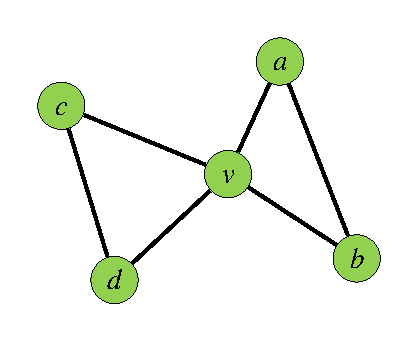
\includegraphics[width=0.36\linewidth]{ego2.pdf}}\label{eego_b}
\subfigure[X-ego network, $\XN{v}$]{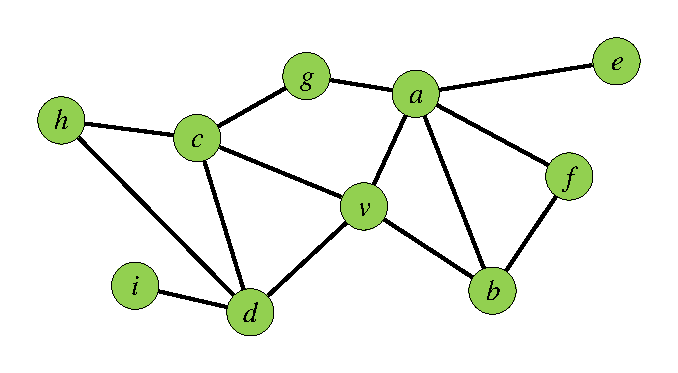
\includegraphics[width=0.6\linewidth]{xego2.pdf}}\label{eego_c}
\caption{Ego and x-ego networks of vertex $v$}
\label{eego2}
\end{figure} 

\begin{center}
\begin{table*}[t]
 \caption{Comparison of betweenness, ego betweenness, and x-ego betweenness for the graph shown in Fig. \ref{eego} (the Pearson correlation is 0.63 between $\B{v}$ and $\BE{v}$ and 0.90 between $\B{v}$ and $\BX{v}$, and the Spearman correlation is 0.79 between $\B{v}$ and $\BE{v}$ and 0.93 between $\B{v}$ and $\BX{v}$)}\label{comparison}
 \resizebox{17.4cm}{!} {
 \begin{tabular}{|c|c|c|c|c|c|c|c|c|c|c|c|c|c|c|}
 \hline
\multicolumn{2}{|c|}{Nodes} & v & a & b & c & d & e & f & g & h & i & j & k & l \\
 \hline
\multirow{2}{*}{$\B{v}$} & Value & 0.405 & 0.383 & 0.124 & 0.131 & 0.286 & 0.000 & 0.318 & 0.049 & 0.030 & 0.167 & 0.000 & 0.000 & 0.000\\
\hhline{~--------------}
& Rank & 1 & 2 & 7 & 6 & 4 & 10 & 3 & 8 & 9 & 5 & 10 & 10 & 10\\
\hhline{---------------}
\multirow{2}{*}{$\BE{v}$} & Value & 0.667 & 0.750 & 0.167 & 0.583 & 0.333 & 0.000 & 0.833 & 1.000 & 0.167 & 0.667 & 0.000 & 0.000 & 0.000\\
\hhline{~--------------}
& Rank & 4 & 3 & 8 & 6 & 7 & 10 & 2 & 1 & 8 & 4 & 10 & 10 & 10\\
\hhline{---------------}
\multirow{2}{*}{$\BX{v}$} & Value & 0.383 & 0.500 & 0.125 & 0.269 & 0.339 & 0.000 & 0.524 & 0.214 & 0.133 & 0.400 & 0.000 & 0.000 & 0.000\\
\hhline{~--------------}
& Rank & 4 & 2 & 9 & 6 & 5 & 10 & 1 & 7 & 8 & 3 & 10 & 10 & 10\\
\hhline{---------------}
 \hline
 \end{tabular}
}
\end{table*}
\end{center}

\vspace{-10mm}In Fig.~\ref{eego2}, $\LV{v}{1} = \V{v}{0} \cup \V{v}{1} = \{v, a, b, c, d\}$ and $\LE{v}{1}=\{ \{v, a\}, \{v, b\}, \{v, c\}, \{v, d\},$ $\{a, b\}, \{c, d\} \}$.
The ego network of vertex $v$, $\EN{v}(\LV{v}{1}, \LE{v}{1})$, is shown in Fig.~\ref{eego2}(a).

Ego networks well model the relationships/interactions between a node and others in a social graph.
However, ego networks have the limitation that it does not capture a substantial amount of information.
For example, in Fig.~\ref{eego2}, assume that node $v$ received from node $a$ the information about $a$'s 1-hop neighbors (i.e., $b$, $e$, $f$, $g$, and $v$).
Despite this information, the ego network of $v$ cannot record the social links between $a$ and $e$, between $a$ and $f$, and between $a$ and $g$ since it can represent only the social links between $v$ and the 1-hop neighbors of $v$.

To overcome the above limitation, we introduce the following extension to ego networks:

\begin{definition}\label{def:xego-network}
Given a graph $G(V, E)$ and a vertex $v \in V$, the \emph{n-layered ego network} of $v$ is $\ENN{v}{n}(\LV{v}{n}, \LE{v}{n} - \E{v}{n})$, where $\LV{v}{2}$ is the set of vertices that are at most 2 hops away from $v$, $\LE{v}{2}$ is the set of edges between vertices that are at most 2 hops away from $v$, and $\E{v}{2}$ is the set of edges between 2-hop neighbors of $v$.
\end{definition}

% For example, the x-ego network of the node represented by vertex 0 is  $\XN{0} (V_{2}^{0}$, $E_{2}^{0} \cup E_{1 \mhyphen 1}^{0})$ shown in Fig.~\ref{eego} (c). x-ego networks are different from 2nd order ego networks (or friends of friends) of which edge sets includes $E_{2 \mhyphen 2}^{v}$ as well as $E_{2}^{v} \cup E_{1 \mhyphen 1}^{v}$. 
% 
% Note that the vertex and edge sets of an x-ego network $\XN{v}$ for a vertex $v$ are also defined as follows:
% \begin{eqnarray}\label{chi}
% V_{2}^{v} &=& \bigcup_{n \in N_{1}^{v}} V_{1}^{n},\\
% E_{2}^{v} \cup E_{1 \mhyphen 1}^{v} &=& \bigcup_{n \in N_{1}^{v}} E_{1}^{n}.
% \end{eqnarray} It means that a vertex $v$ can generate its x-ego network by using the neighbor information of its neighbors. In summary, both ego and x-ego networks can be obtained with the same (similar) network overhead.
% However, expanded ego networks inherently contain substantially larger amounts of information than ego networks.
% As experimentally demonstrated in Section~\ref{experiments}, highly accurate betweenness centrality values can be obtained from x-ego networks than ego networks.

Fig.~\ref{eego2}(b) shows the x-ego network of $v$ from the graph in Fig.~\ref{eego}.
As Fig.~\ref{eego2}(a) and Fig.~\ref{eego2}(b) illustrate, the x-ego network of $v$ is different from the ego network of $v$ in that it contains 2-hop neighbors of $v$ (i.e., $\LV{v}{2} - \LV{v}{1} = \V{v}{2}$) as well as the edges between a 1-hop neighbor and a 2-hop neighbor of $v$.
Despite this difference, both the ego and x-ego networks of $v$ can be obtained with the same network overhead (since they consume the same messages from 1-hop neighbors of $v$).
The benefits of x-ego networks over ego networks are further verified in Section~\ref{evaluation}.

% For a given graph $G(V, E)$ and an arbitrary vertex $v$, we define the following terms:
% \begin{itemize}
% \item $V_{i}^{v}$: the set of vertices whose shortest distance from $v$ is no larger than $i$ (hence, $V_{0}^{v}=\{v\}$).
% \item $E_{i}^{v}$: the set of edges on shortest paths from $v$ to a node in $V_{i}^{v}$ (hence, $E_{0}^{v}=\emptyset$).
% \item $E_{i \mhyphen j}^{v}$: the set of edges between an $i$-hop neighbor and a $j$-hop neighbor of $v$ (hence, $E_{0 \mhyphen 0}^{v}=\emptyset$).
% \item $N_{i}$: the set of 1-hop neighbor nodes with a direct link to $v_i$.
% \item $E_{i}$: the set of links between $v_i$ to the nodes in $N_{i}$.
% \item $\bar{E}_{i}$: the set of links among the nodes in $N_{i}$.
% \end{itemize} 

%The ego network model has been frequently used in many network analysis. The ego network is the network consisting of a single node(ego) together with the 1st-hop neighbor nodes they are connected to and all the links among those neighbors.
% We also define the following additional terms:
% \begin{itemize}
% \item $N^{2}_{i}$: the set of $v_i$'s 2-hop neighbor nodes each of which has a direct link to a node in $N_{i}$.
% \item $E^{2}_{i}$: the set of links connecting the $N_{i}$ nodes to the $N^{2}_{i}$ nodes.
% %\item $\ddot{E}_{N^{2}_{i}}$: the set of edges of nodes belong to $N^{2}_{i}$.
% \end{itemize} 

\subsection{Ego and X-Ego Betweenness}\label{betweenness}

% In much literature, the betweenness $C_{B}(i)$ for a node $v$ has been formally defined as follows:\begin{equation}\label{bet}
% C_{B}(v) = \frac{\sum_{s \neq v \neq t \in V, s<t}\frac{\sigma_{st}(v)}{\sigma_{st}}}{(n-1)(n-2)/2}.
% \end{equation} where $n$ is the total number of nodes, $\sigma_{st}$ is the number of shortest paths from $s$ to $t$, and $\sigma_{st}(i)$ is the number of those shortest paths that include the node $v$. In an undirected network, $\sigma_{st}=\sigma_{ts}$ and $\sigma_{st}(i)=\sigma_{ts}(i)$. The denominator denotes the total number of pairs of nodes except $v$ in an undirected network and normalizes $C_{B}(v)$ to a value between 0 and 1.

In the literature~\cite{centrality, everett, Brandes01afaster}, given a graph $G(V, E)$, the betweenness $\B{v}$ of a vertex $v$ is defined as:
\begin{equation}\label{bet}
\B{v} = \frac{\sum_{s \neq v \neq t \in V}\frac{\sigma_{st}(v)}{\sigma_{st}}}{(|V|-1)(|V|-2)}
\end{equation} where $\sigma_{st}$ is the number of shortest paths from vertex $s$ to vertex $t$ and $\sigma_{st}(v)$ is the number of those shortest paths that pass through vertex $v$. 
% \B{v} = \frac{2 \cdot \sum_{s \neq v \neq t \in V,\ s < t}\frac{\sigma_{st}(v)}{\sigma_{st}}}{(|V|-1)(|V|-2)}.
% \end{equation} where $\sigma_{st}$ is the number of shortest paths from vertex $s$ to vertex $t$ and $\sigma_{st}(v)$ is the number of those shortest paths that pass through vertex $v$. 
In the above definition, the denominator represents the total number of pairs of vertices except $v$.
It normalizes $\B{v}$ to a value between 0 and 1.
Given an undirected graph, $\sigma_{st}=\sigma_{ts}$ and $\sigma_{st}(v)=\sigma_{ts}(v)$ for all vertices $s$, $t$, and $v$.
Therefore, it is sufficient to find either $\sigma_{st}$ or $\sigma_{ts}$ and either $\sigma_{st}(v)$ or $\sigma_{ts}(v)$.

% The globally computed betweenness based on (\ref{bet}) requires much information about the whole network topology and causes large computational and message load overheads. Since a DTN node may be energy-constrained and there is usually no explicit centralized network node in a DTN, such computation is not reasonable. Thus, getting local information from encounter nodes and generating ego or x-ego networks in a distributed way are practically feasible.
% 
% A node $v$'s \emph{ego betweenness} $C^{\mathcal{E}}_{B}(v)$ on its ego network $\EN{v}$ is locally computed as follows:\begin{equation}\label{ebet}
% C^{\mathcal{E}}_{B}(v) = \frac{\sum_{s \neq v \neq t \in V_{1}^{v}, s<t}\frac{\sigma_{st}(v)}{\sigma_{st}}}{(|V_{1}^{v}|-1)(|V_{1}^{v}|-2)/2}. 
% \end{equation} and the \emph{x-ego betweenness} $C^{\mathcal{X}}_{B}(v)$ on its x-ego network $\XN{v}$ is also locally obtained as follows: \begin{equation}\label{eebet}
% C^{\mathcal{X}}_{B}(v) = \frac{\sum_{s \neq v \neq t \in V_{2}^{v}, s<t}\frac{\sigma_{st}(v)}{\sigma_{st}}}{(|V_{2}^{v}|-1)(|V_{2}^{v}|-2)/2}.
% \end{equation} Although the x-ego betweenness requires more computational time than the ego betweenness, it has the similar benefit of simplicity with the ego network in terms of information collection and network configuration. On the other hand, the x-ego betweenness includes more local information than the ego network, so that it will be more accurate than the ego betweenness. 

In a large wireless network, obtaining the betweenness of each node (i.e., the betweenness of the vertex representing that node) is costly since  all nodes that have limited memory and energy must exchange and consume a substantial number of messages to identify the shortest paths between them.
On the other hand, each node can obtain its ego and x-ego networks with much lower overhead since each node  needs to broadcast information about its 1-hop neighbors (Section~\ref{x-ego_definition}). 
In this paper, we consider the situations where each node computes its betweenness using either its ego network or x-ego network and then uses the result as an estimate of its true betweenness in the entire network.
We refer to the betweenness of $v$ computed from the ego network and x-ego network of $v$ as the {\em ego betweenness} and {\em x-ego betweenness} of $v$ (denoted $\BE{v}$ and $\BX{v}$), respectively.

% To compare the accuracy of $\BE{v}$ or $\BX{v}$, we first use the Spearman's rank correlation which measures the {\em monotonic} relationship between the ranked variables of $\BX{v}$ and $\B{v}$ or $\BE{v}$ and $\B{v}$.  The correlation value can vary between -1.0 and +1.0. The closer value is to +1.0, the stronger the association between the values. For the sake of completeness, we also measure the well-known Pearson correlation. The Pearson correlation coefficient assesses a {\em linear} relationship between the two variables and the calculation is based not on the ranked variables, but on the actual betweenness values.

% For the networks shown in Fig. \ref{}, Table \ref{comparison} shows the comparison of globally computed, ego, and x-ego betweenness. Although the actual betweenness values are different with each other, we can see that 1) the rank order of the three betweenness values are very similar to each other, and 2) the rank order of x-ego betweenness is more similar to the one of globally computed betweenness than the one of ego betweenness. We will verify the details with real mobility trace data in Section IV.

Table~\ref{comparison} shows, for every vertex $v$ in Fig.~\ref{eego}, the betweenness ($\B{v}$), ego betweenness ($\BE{v}$), and x-ego betweenness ($\BX{v}$).
In this table, for most of the vertices, x-ego betweenness is closer to betweenness than ego-betweenness mainly because it is derived from a larger number of vertices and edges.
For this reason, the correlation coefficient (also known as the Pearson correlation coefficient) of x-ego betweenness and betweenness (0.9) is higher than that of ego-betweenness and betweenness (0.63).
The advantage of x-ego betweenness over ego betweenness can also be observed in terms of Spearman's rank correlation, which indicates, given two series $\mathcal{X}=(X_1, X_2, \cdots, X_N)$ and $\mathcal{Y}=(Y_1, Y_2, \cdots, Y_N)$, the correlation between $(r_{\mathcal{X}}(X_1), r_{\mathcal{X}}(X_2)$ $, \cdots, r_{\mathcal{X}}(X_N))$ and $(r_{\mathcal{Y}}(Y_1), r_{\mathcal{Y}}(Y_2), \cdots, r_{\mathcal{Y}}(Y_N))$, where $r_{\mathcal{X}}(X_i)$ and $r_{\mathcal{Y}}(Y_i)$ represent the rank of $X_i$ in $\mathcal{X}$ and that of $Y_i$ in $\mathcal{Y}$, respectively.
In Table~\ref{comparison}, Spearman's correlation is 0.93 between x-ego betweenness and betweenness and 0.79 between ego betweenness and betweenness.
In Section~\ref{evaluation}, we further demonstrate the benefit of x-ego betweenness using wireless trace data.

\subsection{Properties of X-Ego Networks}\label{x-go_properties}
In this section, we present four properties of x-ego networks. 
These properties enable efficient x-ego betweenness computation (Section~\ref{computation}). 
As in Brandes' work~\cite{Brandes01afaster}, we denote the \emph{dependency} of vertices $s$ and $t$ on vertex $v$ as $\D{s}{t}{v} = \frac{\sigma_{st}(v)}{\sigma_{st}}$.
Then, the betweenness of $v$ (Equation (\ref{bet})) can be computed by adding the dependency values for all pairs of vertices excluding $v$.
To quickly calculate such dependency values in x-ego networks, we have identified the properties explained below. 

% By Equation (\ref{bet}), we can know that the betweenness of $v$ can be obtained by summing the dependencies for all pairs of vertices, except for $v$, in $\XN{v}$.
% % The exhaustive search of such all shortest paths is computationally expensive. 
% We identify the following properties, {\em Theorem \ref{theorem1}, \ref{theorem2}, \ref{theorem3}}, and  {\em \ref{theorem4}}, to obtain such dependencies with low computational overhead.
% % Therefore, we need to devise {\em skip conditions} or (\ldots) to reduce the computational burden.  
\begin{theorem}
\label{theorem1} 
Assume a vertex $v$, its x-ego network $\XN{v}$, and its two different 1-hop neighbors $s$ and $t$ (i.e., $s, t \in \V{v}{1}$ and $s \ne t$).
Then, $\D{s}{t}{v} = 0$ if there is an edge between $s$ and $t$ (i.e., $\{s, t\} \in \E{v}{1}$).
\begin{proof}
Since $\{s, t\} \in \E{v}{1}$, $d(s, t) = 1$.
Furthermore, $s, t \in \V{v}{1}$, meaning that $d(s, v) + d(v, t) = 1 + 1 = 2 > d(s, t) = 1$ (i.e., no shortest path from $s$ to $t$ passes through $v$).
Therefore, $\D{s}{t}{v} = \sigma_{st}(v)/\sigma_{st} = 0/\sigma_{st} = 0$.\hfill\qed
\end{proof}
\end{theorem}


\begin{example}
In Fig.~\ref{eego2}(b), $\D{a}{b}{v} = 0$ since $a, b \in \V{v}{1}$ and there is an edge between $a$ and $b$.
\end{example}

% Theorem \ref{theorem1} will take on a key role as a computation skipping rule in the algorithm to compute the x-ego betweenness, $\BX{v}$. In particular, it will reduce the computational overload substantially when a vertex $v$'s x-ego network exhibits a strong community structure (i.e., nodes in ego networks tend to interact with each other). Since friends of a friend are likely to be friends as well, we can expect that this transitivity should be frequently observed in x-ego networks derived by a DTN. 
% 
% In case that the skipping rule presented by Theorem \ref{theorem1} cannot be applied for a pair of $v$'s two 1-hop neighbors, the dependency of them is computed by using the following Theorem \ref{theorem2}. 

Theorem \ref{theorem1} allows us to quickly compute dependencies particularly when x-ego networks exhibit a strong community structure (i.e., 1-hop neighbors of a node tend to have direct social links between them).
In Section~\ref{evaluation}, we show this benefit using wireless trace data.

When Theorem \ref{theorem1} cannot be applied to $v$'s 1-hop neighbors $s$ and $t$ (i.e., there is no edge between $s$ and $t$), the dependency of $s$ and $t$ on $v$ can be computed using the following theorem.

\begin{theorem}
\label{theorem2} 
Assume a vertex $v$, its x-ego network $\XN{v}$, and its two different 1-hop neighbors $s$ and $t$ (i.e., $s, t \in \V{v}{1}$ and $s \ne t$).
Then, $\D{s}{t}{v} = {1}/{|\V{s}{1} \cap \V{t}{1}|}$ if there is no edge between $s$ and $t$ (i.e., $\{s, t\} \notin \E{v}{1}$).
\begin{proof}
Since $\{s, t\} \notin \E{v}{1}$, $d(s, t) > 1$.
In this case, $d(s, t) = 2$ due to the path $s - v - t$.
Furthermore, (i) the number of shortest paths from $s$ to $t$ (i.e., paths whose length is 2) can be expressed as $\sigma_{st} = |\V{s}{1} \cap \V{t}{1}|$.
%  indicates the number of shortest paths starting from $v_s \in N_0$ and terminating at $v_t \in N_0$.
On the other hand, (ii) the path $s-v-t$ is the only shortest path from $s$ to $t$ that passes through $v$ (i.e., $\sigma_{st}(v) = 1$) since the length of that path is 2, which must be smaller than the length of any other path from $s$ to $t$ that passes through $v$.
By (i) and (ii), $\D{s}{t}{v} = \sigma_{st}(v)/\sigma_{st} = {1}/{|\V{s}{1} \cap \V{t}{1}|}$.\hfill\qed
\end{proof}
\end{theorem}

% \begin{equation}
% \D{s}{t}{v} =
%   \begin{cases}
%    0       & \text{if $(s, t) \in E$} \\
%    {\displaystyle \frac {1}{|\V{s}{1} \cap \V{t}{1}|}} & \text{ otherwise.} \\
%   \end{cases}
% \end{equation}

\begin{example}
\label{example2} 
In Fig.~\ref{eego2}(b), vertices $a$ and $c$ are 1-hop neighbors of $v$ and there is no edge between $a$ and $c$.
Furthermore, $\V{a}{1} = \lbrace b, e, f, g, v\rbrace$ and $\V{c}{1} = \lbrace d, g, h, v\rbrace$.
Therefore, $\D{a}{c}{v}=1/|\V{a}{1} \cap \V{c}{1}|=1/|\{g, v \}|=1/2$.

% $\LV{a}{1} = \lbrace v, b, e, f, g\rbrace$, $\LV{c}{1} = \lbrace v, d, g, h\rbrace$ and $\LV{d}{1} = \lbrace v, c, h, i\rbrace$. So, node $v$ can get the non-zero $\D{a}{c}{v}=1/2=0.5$ and $\D{a}{d}{v}=1/1=1$ because $v$ knows that $a$ does not share any edge with $c$ and $d$, $|\LV{a}{1} \cap \LV{c}{1}| = |\lbrace v, g\rbrace|=2$, and $|\LV{a}{1} \cap \LV{d}{1}| = |\lbrace v\rbrace$| = 1. 
\end{example}

Just like Theorem~\ref{theorem1}, the following theorem quickly computes the dependency of two vertices on a vertex $v$.
While the former applies to a pair of 1-hop neighbors of $v$, the latter applies to a pair of a 1-hop or 2-hop neighbor and a 2 hop-neighbor of $v$.
% The following Theorem \ref{theorem3} presents another skipping rule to reduce the computation overload of the dependency for an 1 or 2-hop neighbor and a 2-hop neighbor of $v$.

\begin{theorem}
\label{theorem3} 
Assume a vertex $v$, its x-ego network $\XN{v}$, a vertex $s \in \LV{v}{2}$, and another vertex $t \in \V{v}{2}$ such that $s \ne t$.
Then, $\D{s}{t}{v} = 0$ if $\D{s}{n}{v} = 0$ for a 1-hop neighbor vertex $n$ of vertex $t$ (i.e., for $n \in \V{t}{1}$).
\begin{proof}
Since $\D{s}{n}{v} = 0$ (i.e., no shortest path from $s$ to $n$ passes through $v$), (i) $d(s, n) < d(s, v) +d(v, n)$.
Then, (ii) $d(s, t) \le d(s, n) + d(n, t) < d(s, v) + d(v, n) + d(n, t)$ by (i).
Furthermore, $n \in \V{t}{1}$ and $t \in \V{v}{2}$, meaning that vertex $n$ is either a 1-hop or a 3-hop neighbor of $v$.
In $\XN{v}$, however, any vertex including $n$ is at most 2 hops away from $v$.
For this reason, $n$ is a 1-hop neighbor of $v$.
Since $d(v, n)$=$d(n, t)$=$1$ and $d(v, t)=2$, (iii) $d(v, n) + d(n, t) = d(v, t)$. 
By (ii) and (iii), $d(s, t) < d(s, v) +d(v, t)$ (i.e., no shortest path from $s$ to $t$ passes through $v$).
Therefore, $\D{s}{t}{v}  = \sigma_{st}(v)/\sigma_{st} = 0/\sigma_{st} = 0$.\hfill\qed
\end{proof}
\end{theorem}

\begin{example}
In Fig. \ref{eego2}(b), $b \in \LV{v}{2}$ and $g \in \V{v}{2}$. 
Furthermore, for a 1-hop neighbor $a$ of $g$, $\D{b}{a}{v}=0$ (Theorem \ref{theorem1}).
Therefore, by Theorem \ref{theorem3}, $\D{b}{g}{v}=0$.
\end{example}

Given vertices $s \in \LV{v}{2}$ and $t \in \V{v}{2}$ such that $s \ne t$, Theorem~\ref{theorem3} cannot be applied if $\D{s}{n}{v} > 0$ for every 1-hop neighbor $n$ of $t$.
In this case, the dependency of $s$ and $t$ on $v$ can be obtained using the following theorem.
% Lastly, the following Theorem \ref{theorem4} presents that the harmonic mean can be used to compute the dependency for an 1 or 2-hop neighbor and a 2-hop neighbor of $v$, if they do not satisfy the condition of Theorem \ref{theorem3}. 

\begin{theorem}
\label{theorem4} 
Assume a vertex $v$, its x-ego network $\XN{v}$, a vertex $s \in \LV{v}{2}$, and another vertex $t \in \V{v}{2}$ such that $s \ne t$.
Then, $\D{s}{t}{v} = \bar{H}(\{\D{s}{n}{v} : n \in \V{t}{1}\})$ if $\D{s}{n}{v} > 0$ for every 1-hop neighbor $n$ of vertex $t$, where $\bar{H}(\{\D{s}{n}{v} : n \in \V{t}{1}\})$ denotes the {\em harmonic mean} computed over $\{\D{s}{n}{v} : n \in \V{t}{1}\}$.
\begin{proof}
We prove this theorem considering the following two cases.
% in two cases, $s \in \LV{v}{1}$ or $s \in \LV{v}{2}-\LV{v}{1}$, separately:

\noindent [Case I. $s$ is a 1-hop neighbor of $v$ (i.e., $s \in \V{v}{1}$)]
% Let us assume there are $m$ 1-hop neighbors of $t$ in $\XN{v}$ and let $n_i$ denote the $i$th 1-hop neighbor of $t$ such that $\D{s}{n_i}{v} > 0$. In $\XN{v}$, each $n_i$ is also an 1-hop neighbor of $v$ (i.e., $n_i \in \LV{v}{1}$) and $\D{s}{n_i}{v} = {1}/{|\LV{s}{1} \cap \LV{n_i}{1}|}$ by Theorem \ref{theorem2}. 
% Furthermore, (i) $|\LV{s}{1} \cap \LV{n_i}{1}|=1/\D{s}{n_i}{v}$ represents the number of shortest paths from $s$ to $n_i$ (i.e., $\sigma_{sn_i}$) and the total number of shortest paths from $s$ to $t$ can be expressed as $\sigma_{st} = \sum_{i=1}^m 1/\D{s}{n_i}{v}$ since each $n_i$ shares an edge with $t$. On the other hand, (ii) the path $s-v-n_i-t$ is the only shortest path from $s$ to $t$ via both $v$ and $n_i$ since the length of the path is 3 and any other path from $s$ to $t$ via both $v$ and $n_i$ must be longer. It means that there are $m$ shortest paths from $s$ to $t$ via $v$ (i.e., $\sigma_{st}(v)=m$). By (i) and (ii), $\D{s}{t}{v} = \frac{m}{\sum_{i=1}^m 1/\D{s}{n_i}{v}} = \bar{H}(\D{s}{n}{v})$.
Let $n_i$ ($i=1,2,\cdots, m$) denote the $i$th 1-hop neighbor of $t$.
Then, each $n_i$ is a 1-hop neighbor of $v$ since, in $\XN{v}$, any 2-hop neighbor (including $t$) of $v$ can be connected only to a 1-hop neighbor of $v$ (Definition~\ref{def:xego-network}).
Thus, by Theorem \ref{theorem2}, $\D{s}{n_i}{v} = {1}/{|\V{s}{1} \cap \V{n_i}{1}|}$. 
Since $|\V{s}{1} \cap \V{n_i}{1}|$ represents the number of shortest paths from $s$ to $n_i$ (i.e., $\sigma_{sn_i}$) and each $n_i$ has an edge to $t$, the total number of shortest paths from $s$ to $t$ can be expressed as (i) $\sigma_{st} = \sum_{i=1}^m |\V{s}{1} \cap \V{n_i}{1}| = \sum_{i=1}^m 1/\D{s}{n_i}{v}$. 
On the other hand, the path $s-v-n_i-t$ is the only shortest path from $s$ to $t$ via both $v$ and $n_i$ since the length of the path is 3 and any other path from $s$ to $t$ via both $v$ and $n_i$ must be longer.
For this reason, (ii) there are $m$ shortest paths from $s$ to $t$ via $v$ (i.e., $\sigma_{st}(v)=m$).
By (i) and (ii), $\D{s}{t}{v} = \frac{m}{\sum_{i=1}^m 1/\D{s}{n_i}{v}} = \bar{H}(\D{s}{n}{v})$.

\noindent [Case II. $s$ is a 2-hop neighbor of $v$ (i.e., $s \in \V{v}{2}$)]
Let $n_i~(i=1,2,\cdots,m)$ denote the $i$th 1-hop neighbor of $t$. 
Let also $p_j~(j=1,2,\cdots,k)$ denote the $j$th 1-hop neighbor of $s$.
In $\XN{v}$, 2-hop neighbors (including $s$ and $t$) of $v$ can be connected only to a 1-hop neighbor of $v$.
For this reason, any shortest path from $s$ to $t$ must contain a shortest path from $p_j$ to $n_i$ for some $j$ and $i$ 
% Since $n_i$ and $p_j$ respectively shares an edge with $t$ and $s$, the shortest path from $n_i$ to $n_j$ for a pair of $i$ and $j$ always corresponds to the one from $s$ to $t$ 
(i.e., $\sigma_{st} = \sum_{i=1}^m \sum_{j=1}^k |\V{n_i}{1} \cap \V{p_j}{1}|$). 
For a pair of $i$ and $j$, on the other hand, the path $n_i-v-p_j$ is the only shortest path from $n_i$ to $p_j$ via $v$ and so is the path $t-n_i-v-p_j-s$ (i.e., $\sigma_{st}(v)=mk$). 
Therefore, 
\begin{eqnarray}
\D{s}{t}{v} 
&=& \frac{mk}{\sum_{i=1}^m \sum_{j=1}^k |\V{n_i}{1} \cap \V{p_j}{1}|} \nonumber \\ 
&=& \frac{mk}{\sum_{i=1}^m \sum_{j=1}^k 1/\D{n_i}{p_j}{v}} \nonumber \\ 
&=& \frac{m}{\sum_{i=1}^m \frac {\sum_{j=1}^k 1/\D{n_i}{p_j}{v}}{k}} \nonumber \\ 
&=& \frac{m}{\sum_{i=1}^m 1/\D{n_i}{s}{v}} \nonumber \\ 
&=& \frac{m}{\sum_{i=1}^m 1/\D{s}{n_i}{v}} \nonumber  \\
&=& \bar{H}(\D{s}{n}{v}).   \nonumber
\end{eqnarray}\qed
\label{harmonic_eq}
\end{proof}
\end{theorem}

% \label{harmonic} 
% For a vertex $v$, its x-ego network $\XN{v}$, a vertex $s \in \V{v}{1} \cup \V{v}{2}$ and another vertex $t \in \V{v}{2}$, let $n_1, n_2, \cdots, n_i$ ($n_i \leq u$) denote the 1-hop neighbor vertices of vertex $t$. 
% Then, 
% \begin{equation}
% \D{s}{t}{v} =
%   \begin{cases}
%    0      &\text{if $\exists k, \D{s}{n_k}{v} = 0$} \\
%    \bar H (\D{s}{n_k}{v}) &\text{otherwise.}
%    \end{cases}
% \end{equation} where $\bar H_{st}$ is the harmonic mean for all the non-zero $f_{s{n_k}}$ values.
% \end{theorem}
% \begin{proof}
% ...\\
% ...\\
% ...\\
% ... \qed
% \end{proof}
\begin{example}
In Fig.~\ref{eego2}(b), % consider the dependency $\D{a}{h}{v}$ of $a \in \LV{v}{2}$ and $h \in \V{v}{2}$ on $v$. In this example, 
$\V{h}{1} = \{c,d\}$.
By Theorem \ref{theorem2}, $\D{a}{c}{v}=\frac{1}{2}$ and $\D{a}{d}{v}=1$.
Therefore, by Theorem \ref{theorem4}, $\D{a}{h}{v}\!=\!\bar{H}(\{\D{a}{n}{v} : n \in \V{h}{1}\})\!=\!\bar{H}(\{\D{a}{c}{v},\D{a}{d}{v}\})\!=\!\frac{2}{\frac{1}{\frac{1}{2}} + \frac{1}{1}}=\frac{2}{3}$.  
 
% For each 1-hop neighbor $n$ of $h$ (i.e., $n \in \V{h}{1} = \{ c,d\}$,  and from Theorem \ref{theorem2} it also knows $\D{a}{c}{v}=1/2$ and $\D{a}{d}{v}=1/1$ for $h$'s two 1-hop neighbors, $c$ and $d$. Therefore, we can get $\D{a}{h}{v}$=$\bar{H}(\D{a}{c}{v},\D{a}{d}{v})$=$2/3$. 
% Similarly, $\D{c}{e}{v}=\bar{H}(\D{c}{a}{v})=1/2$ where $c \in \LV{v}{1} (\subset \LV{v}{2})$ and $e \in \LV{v}{2}-\LV{v}{1}$, since $\LV{e}{1}=\{e,a\}$, $\D{c}{a}{v}=1/2$ and $\bar{H}(\D{c}{a}{v})=\D{c}{a}{v}$.
\end{example}

% These four properties will be used in the algorithm proposed in Section \ref{computation} to compute the x-ego betweenness of a DTN node.



\section{Conclusion}
The conclusion goes here.





% if have a single appendix:
%\appendix[Proof of the Zonklar Equations]
% or
%\appendix  % for no appendix heading
% do not use \section anymore after \appendix, only \section*
% is possibly needed

% use appendices with more than one appendix
% then use \section to start each appendix
% you must declare a \section before using any
% \subsection or using \label (\appendices by itself
% starts a section numbered zero.)
%


\appendices
\section{Proof of the First Zonklar Equation}
Appendix one text goes here.

% you can choose not to have a title for an appendix
% if you want by leaving the argument blank
\section{}
Appendix two text goes here.


% use section* for acknowledgment
\section*{Acknowledgment}


The authors would like to thank...


% Can use something like this to put references on a page
% by themselves when using endfloat and the captionsoff option.
\ifCLASSOPTIONcaptionsoff
  \newpage
\fi



% trigger a \newpage just before the given reference
% number - used to balance the columns on the last page
% adjust value as needed - may need to be readjusted if
% the document is modified later
%\IEEEtriggeratref{8}
% The "triggered" command can be changed if desired:
%\IEEEtriggercmd{\enlargethispage{-5in}}

% references section

% can use a bibliography generated by BibTeX as a .bbl file
% BibTeX documentation can be easily obtained at:
% http://mirror.ctan.org/biblio/bibtex/contrib/doc/
% The IEEEtran BibTeX style support page is at:
% http://www.michaelshell.org/tex/ieeetran/bibtex/
\bibliographystyle{IEEEtran}
% argument is your BibTeX string definitions and bibliography database(s)
\bibliography{linkPaper}
%
% <OR> manually copy in the resultant .bbl file
% set second argument of \begin to the number of references
% (used to reserve space for the reference number labels box)

% biography section
% 
% If you have an EPS/PDF photo (graphicx package needed) extra braces are
% needed around the contents of the optional argument to biography to prevent
% the LaTeX parser from getting confused when it sees the complicated
% \includegraphics command within an optional argument. (You could create
% your own custom macro containing the \includegraphics command to make things
% simpler here.)
%\begin{IEEEbiography}[{\includegraphics[width=1in,height=1.25in,clip,keepaspectratio]{mshell}}]{Michael Shell}
% or if you just want to reserve a space for a photo:

\begin{IEEEbiography}{Michael Shell}
Biography text here.
\end{IEEEbiography}

% if you will not have a photo at all:
\begin{IEEEbiographynophoto}{John Doe}
Biography text here.
\end{IEEEbiographynophoto}

% insert where needed to balance the two columns on the last page with
% biographies
%\newpage

\begin{IEEEbiographynophoto}{Jane Doe}
Biography text here.
\end{IEEEbiographynophoto}

% You can push biographies down or up by placing
% a \vfill before or after them. The appropriate
% use of \vfill depends on what kind of text is
% on the last page and whether or not the columns
% are being equalized.

%\vfill

% Can be used to pull up biographies so that the bottom of the last one
% is flush with the other column.
%\enlargethispage{-5in}



% that's all folks
\end{document}


